
\begin{frame}{Proposed Method}
 
    \textbf{Convolutional Neural Networks} $\rightarrow$ poor localization around object boundaries 
    
    \textbf{Active Contour Models} $\rightarrow$ sensitive to initialization, but topologically flexible

    \textbf{Integrated approach} $\rightarrow$ incorporating both high-level and low-level image information

    \vfill
    {\centering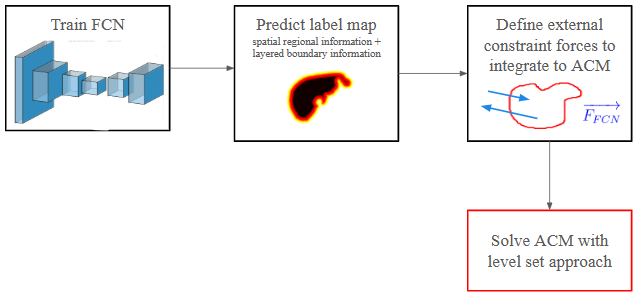
\includegraphics[width=.9\textwidth]{methods.png}}

    \citeall{guo_automatic_2019}
\end{frame}


\subsection{Generate layered label map containing rich information}
\begin{frame}{Generate layered label map containing rich information}
    \begin{columns}
        \begin{column}{.4\textwidth}
            For $7$ layers
            \begin{align*}
                L_{\blue{-3}} &= \lbrace X | \infty < \varphi(X) < -2.5 \delta \rbrace \\
                L_{\blue{-2}} &= \lbrace X | -2.5 \delta < \varphi(X) \leq -1.5 \delta \rbrace \\
                L_{\blue{-1}} &= \lbrace X | -1.5 \delta < \varphi(X) \leq -0.5 \delta \rbrace \\
                L_{0} &= \lbrace X | -0.5 \delta < \varphi(X) \leq 0.5 \delta \rbrace \\
                L_{\orange{1}} &= \lbrace X | 0.5 \delta < \varphi(X) \leq 1.5 \delta \rbrace \\
                L_{\orange{2}} &= \lbrace X | 1.5 \delta < \varphi(X) \leq 2.5 \delta \rbrace \\
                L_{\orange{3}} &= \lbrace X | 2.5 \delta < \varphi(X) \leq \infty \rbrace
            \end{align*}
            $\delta = d/\textrm{ps}$ is a parameter to control narrow bandwidth, $\textrm{ps}$ is the pixel spacing and $d$ is the bandwidth in millimeters
            \tiny{\grey{$d=5$}}
        \end{column}
    \hspace{.8cm}
    \begin{column}{.6\textwidth}
    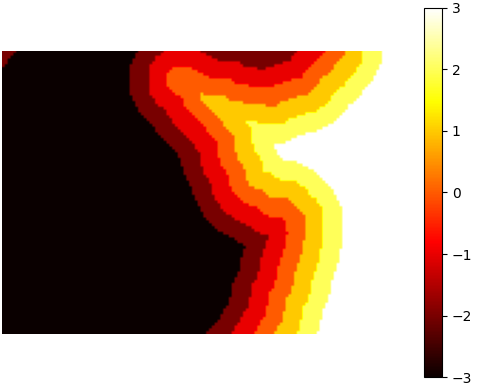
\includegraphics[width=.8\textwidth]{illu_layered_label_map.png}
    \end{column}
    \end{columns}
\end{frame}

\subsection{Train FCN to predict layered label map}
\begin{frame}{Train FCN to predict layered label map}
    Pre-trained model FCN-8 on the PASCAL dataset (21 classes)
     
    {\centering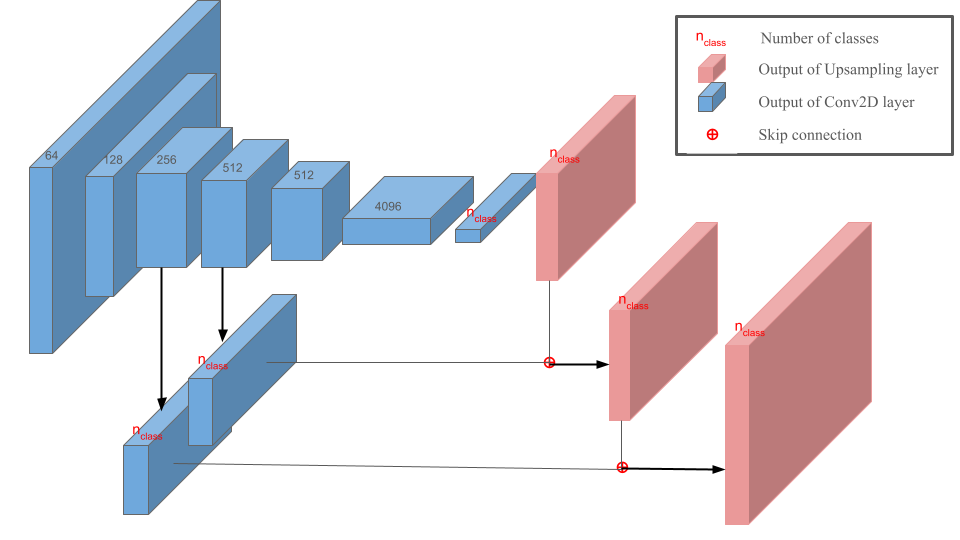
\includegraphics[width=\textwidth]{architecture.png}}
    \citeall{long_fully_2015}
\end{frame}

\subsection{Integrating NN's output to ACM}
\begin{frame}{Active Contour Models}
Let $\varphi$ be a Lipschitz function

Evolving the curve $C = \ens{(x, y)}{\varphi(x, y) = 0} $ in the normal direction with speed $V$ amount to solve 
$$
\left\lbrace \begin{array}{l}
    \frac{\partial \varphi}{\partial t} = V\norm{\nabla \varphi} \\
    \varphi(0, x, y) = \varphi_0(x, y) 
\end{array}
\right.
$$ 
$\varphi_0$ is the signed distance to the initial contour defined by the user

\citeall{chan_active_2001} 
\end{frame}